\input{head.inc}

% Präambelbefehle für die Präsentation
\title[TET: Begriffsbestimmung]{Begriffsbestimmung}

\begin{document}
\maketitle

\section{Begriffsbestimmung}

\begin{frame}
  \frametitle{Was ist Theoretische Elektrotechnik?}
\centerline{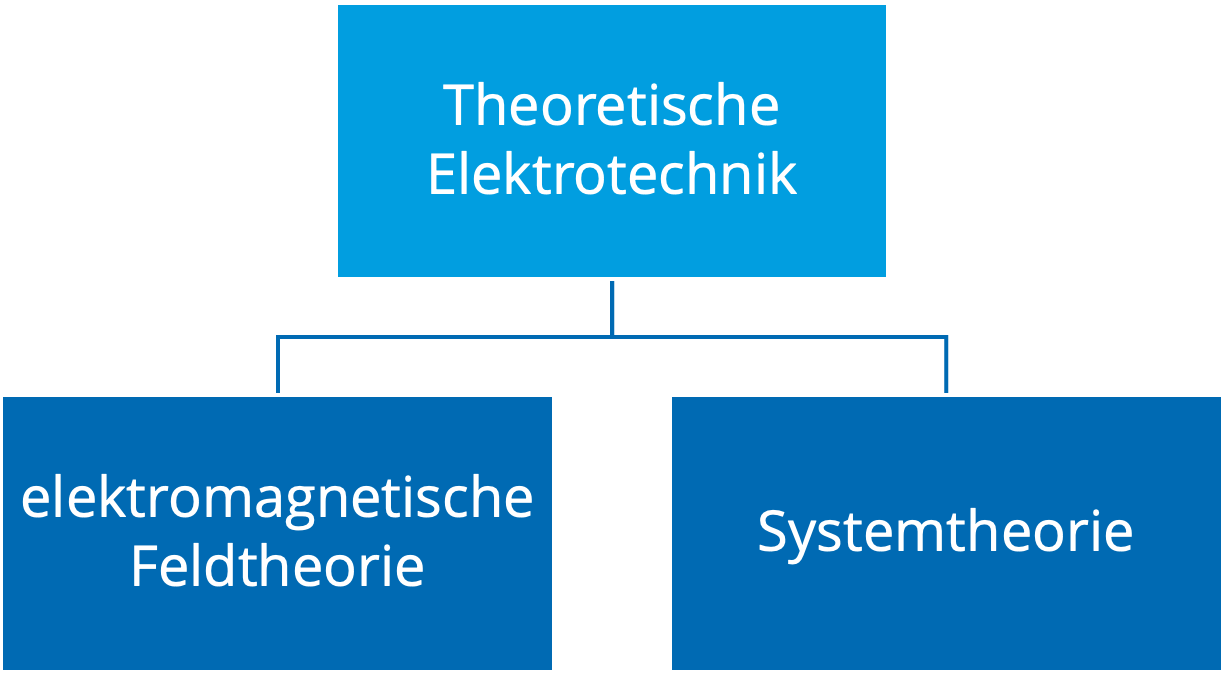
\includegraphics[height=.4\textheight]{TET-Begriff}}

\begin{itemize}[<+->]
\item Die \textbf{Theoretische Elektrotechnik} beinhaltet die \textbf{elektromagnetische Feldtheorie} und die \textbf{Systemtheorie}
  \item TET beschäftigt sich mit den theoretischen Grundlagen der Elektrotechnik; Anwendungen folgen hieraus
\item TUD: Systemtheorie ist eigenes Modul im Studiengang Elektrotechnik \(\to\) kann hier ausgeklammert werden
\item Elektromagnetische Feldtheorie baut auf den \textbf{Maxwellschen Gleichungen} auf
\end{itemize}
\end{frame}

\begin{frame}
  \frametitle{Theoretische Grundlagen -- Was ist eine Theorie?}
\begin{itemize}[<+->]
\item In der Wissenschaft ist Theorie ist nicht das Gegenteil von Praxis!
\item Allgemeiner Sprachgebrauch:
\begin{itemize}[<+->]
\item Theorie = unbewiesene These
\end{itemize}
\item Wissenschaft:
\begin{itemize}[<+->]
\item Theorie = \textbf{System wissenschaftlich begründeter Aussagen}, das dazu dient, \textbf{Ausschnitte der Realität} und die\textbf{ zugrundeliegenden Gesetzmäßigkeiten} zu \textbf{erklären} und \textbf{Prognosen abzuleiten}
  
\item Abgrenzung zum Modell: \textbf{Modelle} dienen häufig der \textbf{Beschreibung bekannter Sachverhalte}. Hierzu \textbf{vereinfachen} Sie das reale Problem oft (z.B. Planetenmodell des Atoms, homogenes Medium) oder gehen von \textbf{idealisierten} Annahmen aus (z.B. ideales Gas, Massenpunkt).
  
\item \textbf{Modelle liefern keine Erklärungen}, unterstützen aber oft den Prozess der Theoriebildung und helfen bei der Veranschaulichung 

\item Erst die Beherrschung einer Theorie ermöglicht die Entwicklung bzw. die Weiterentwicklung von Modellen für neue Problemstellungen. Gleiches gilt für (neue) numerische Berechnungsverfahren.    

\end{itemize}
\end{itemize}
\end{frame}

\begin{frame}
  \frametitle{Erkenntnisprozess}
\centerline{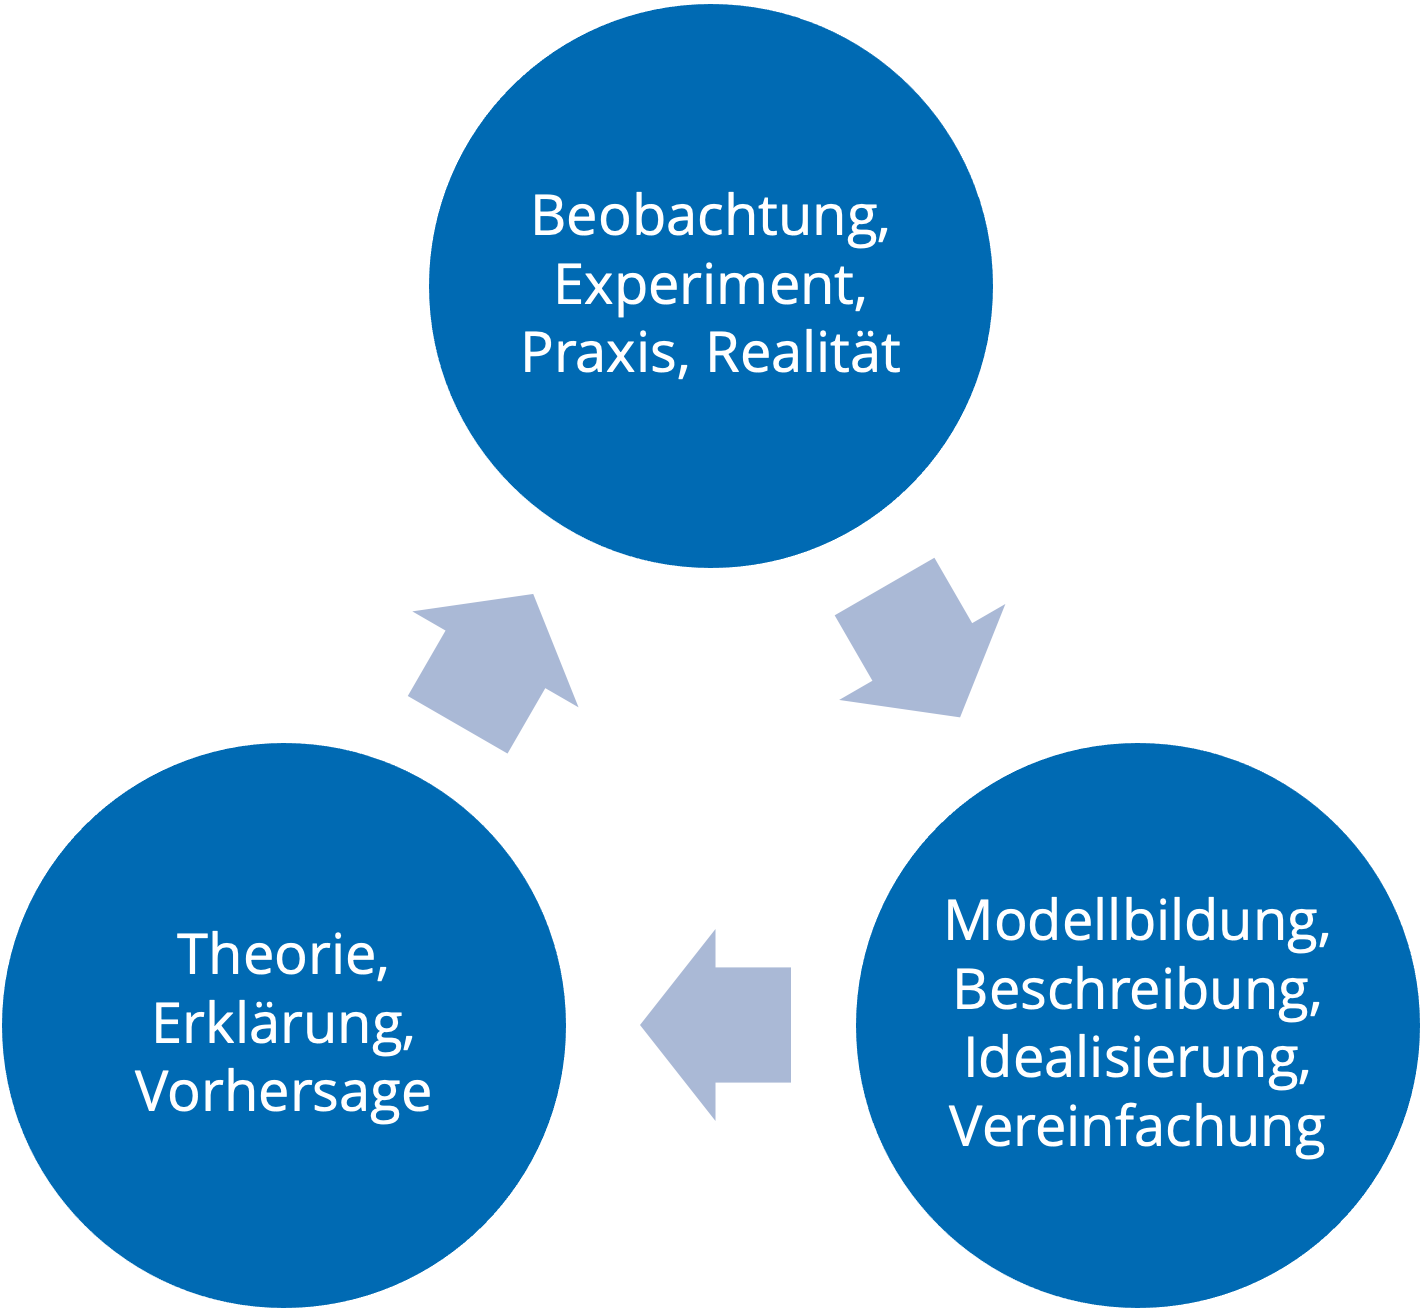
\includegraphics[height=.8\textheight]{TET-Erkenntnisprozess}}

\end{frame}


\input{finalframe.inc}
\end{document}